\section{Giới thiệu}

\begin{frame}{Động lực nghiên cứu}
	\vspace{5pt}
	
	\begin{columns}
	% Left column
	\begin{column}{0.7\textwidth}
		\textbf{Text-base Deep Learning}
		\begin{itemize}
			\item ChatGPT, Alexa, Character.AI,..
			\item Text to speech, text to text,..
		\end{itemize}
		
		\textbf{Text/audio to Realistic Digital Humam}
		
		\begin{itemize}
			\item Video-base (HeyGen, Midjourney,...)
			\item Rendering-base:
			\begin{itemize}
				\item Character model (Gaussian Splatting)
				\item Character animation: (3D keypoints)
			\end{itemize}
		\end{itemize}
		\vspace{5pt}
		\centering
		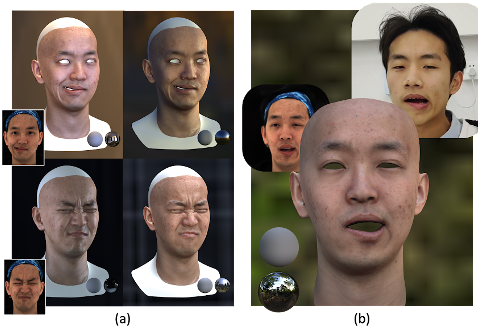
\includegraphics[width=0.8\textwidth]{FacialAsset.png}
	\end{column}
	
	% Right column
	\begin{column}{0.3\textwidth}
		\begin{figure}
				
\includegraphics[width=\textwidth]{UniversalHuman.png}
%				\caption{\small Minh hoạ người kỹ thuật số siêu thật (realistic digital human)}
		\end{figure}
		
		\begin{figure}
			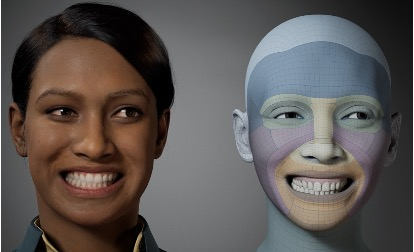
\includegraphics[width=\textwidth]{MetaHuman.jpg}
			\caption{\small Minh hoạ người kỹ thuật số siêu thật (realistic digital human)}
		\end{figure}
	
	\end{column}
	
	\end{columns}
\end{frame}

\begin{frame}
	\begin{columns}
		\begin{column}{0.6\textwidth}
			\centering
			{\Large
			$\{ \mathbf{b}_1, \cdots \mathbf{b}_{75} \}$}
			\vspace{10pt}
			
			\begin{figure}[H]
				\centering
				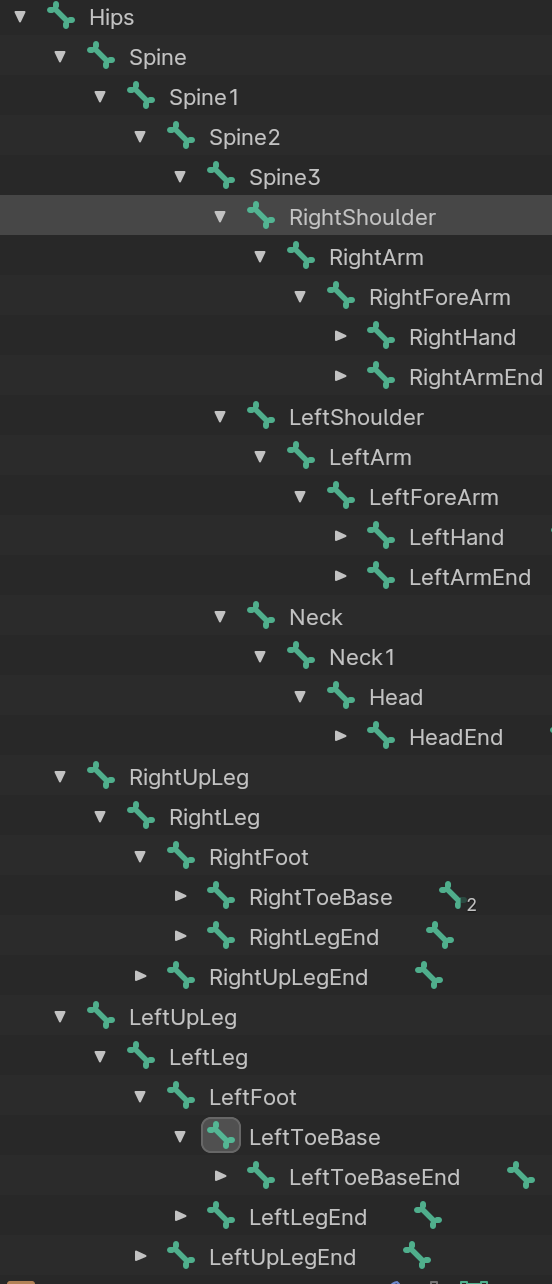
\includegraphics[width=.5\textwidth]{Bone}
			\end{figure}
			
			\vspace{10pt}
			{\Large
				$\mathbf{b}_{i} = \{p_x, p_y, p_z, r_x, r_y, r_z\}$}
		\end{column}
		
		\begin{column}{0.4\textwidth}
			\begin{figure}[h]
				\centering
				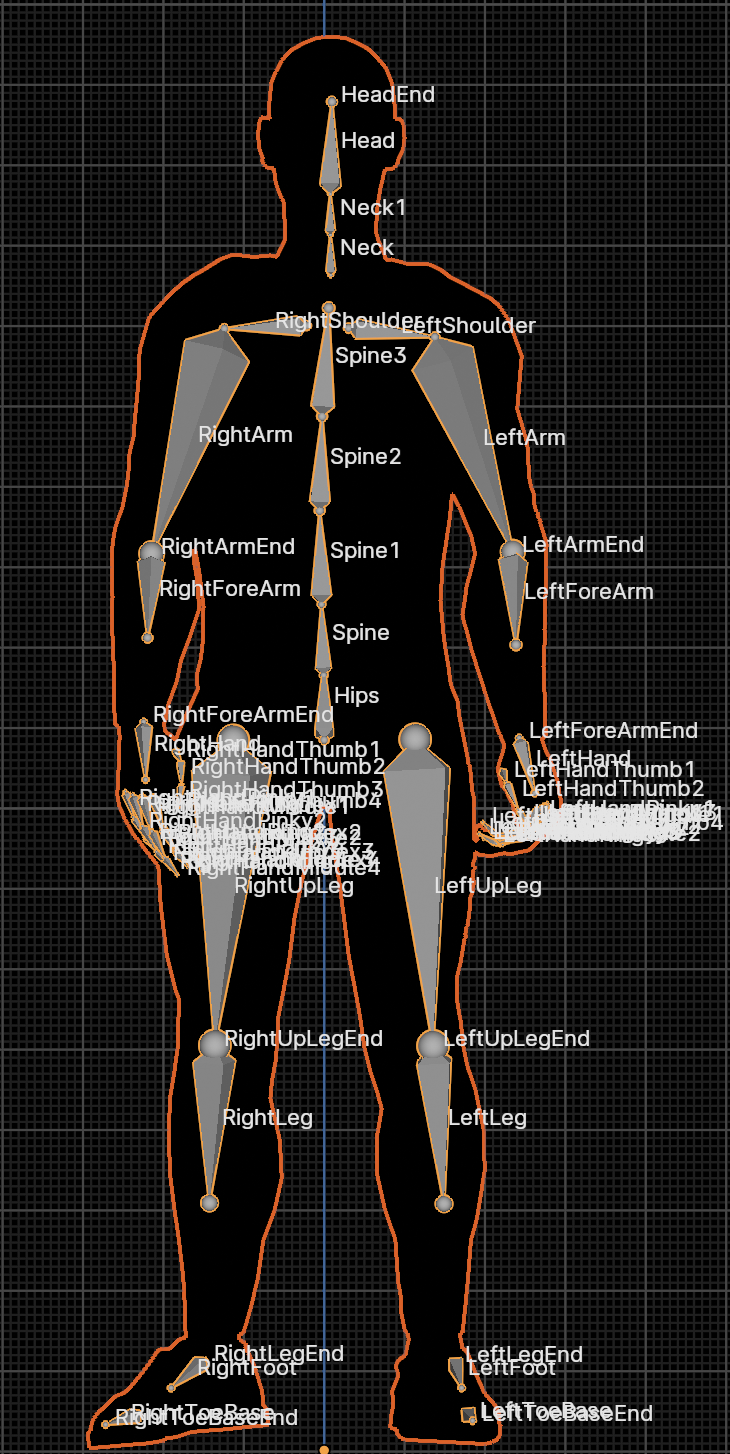
\includegraphics[width=\textwidth]{Skeleton}
			\end{figure}
		\end{column}
		
	\end{columns}
	
\end{frame}

%Dữ liệu cử chỉ cần học
\begin{frame}
		\begin{figure}[h]
		\centering
		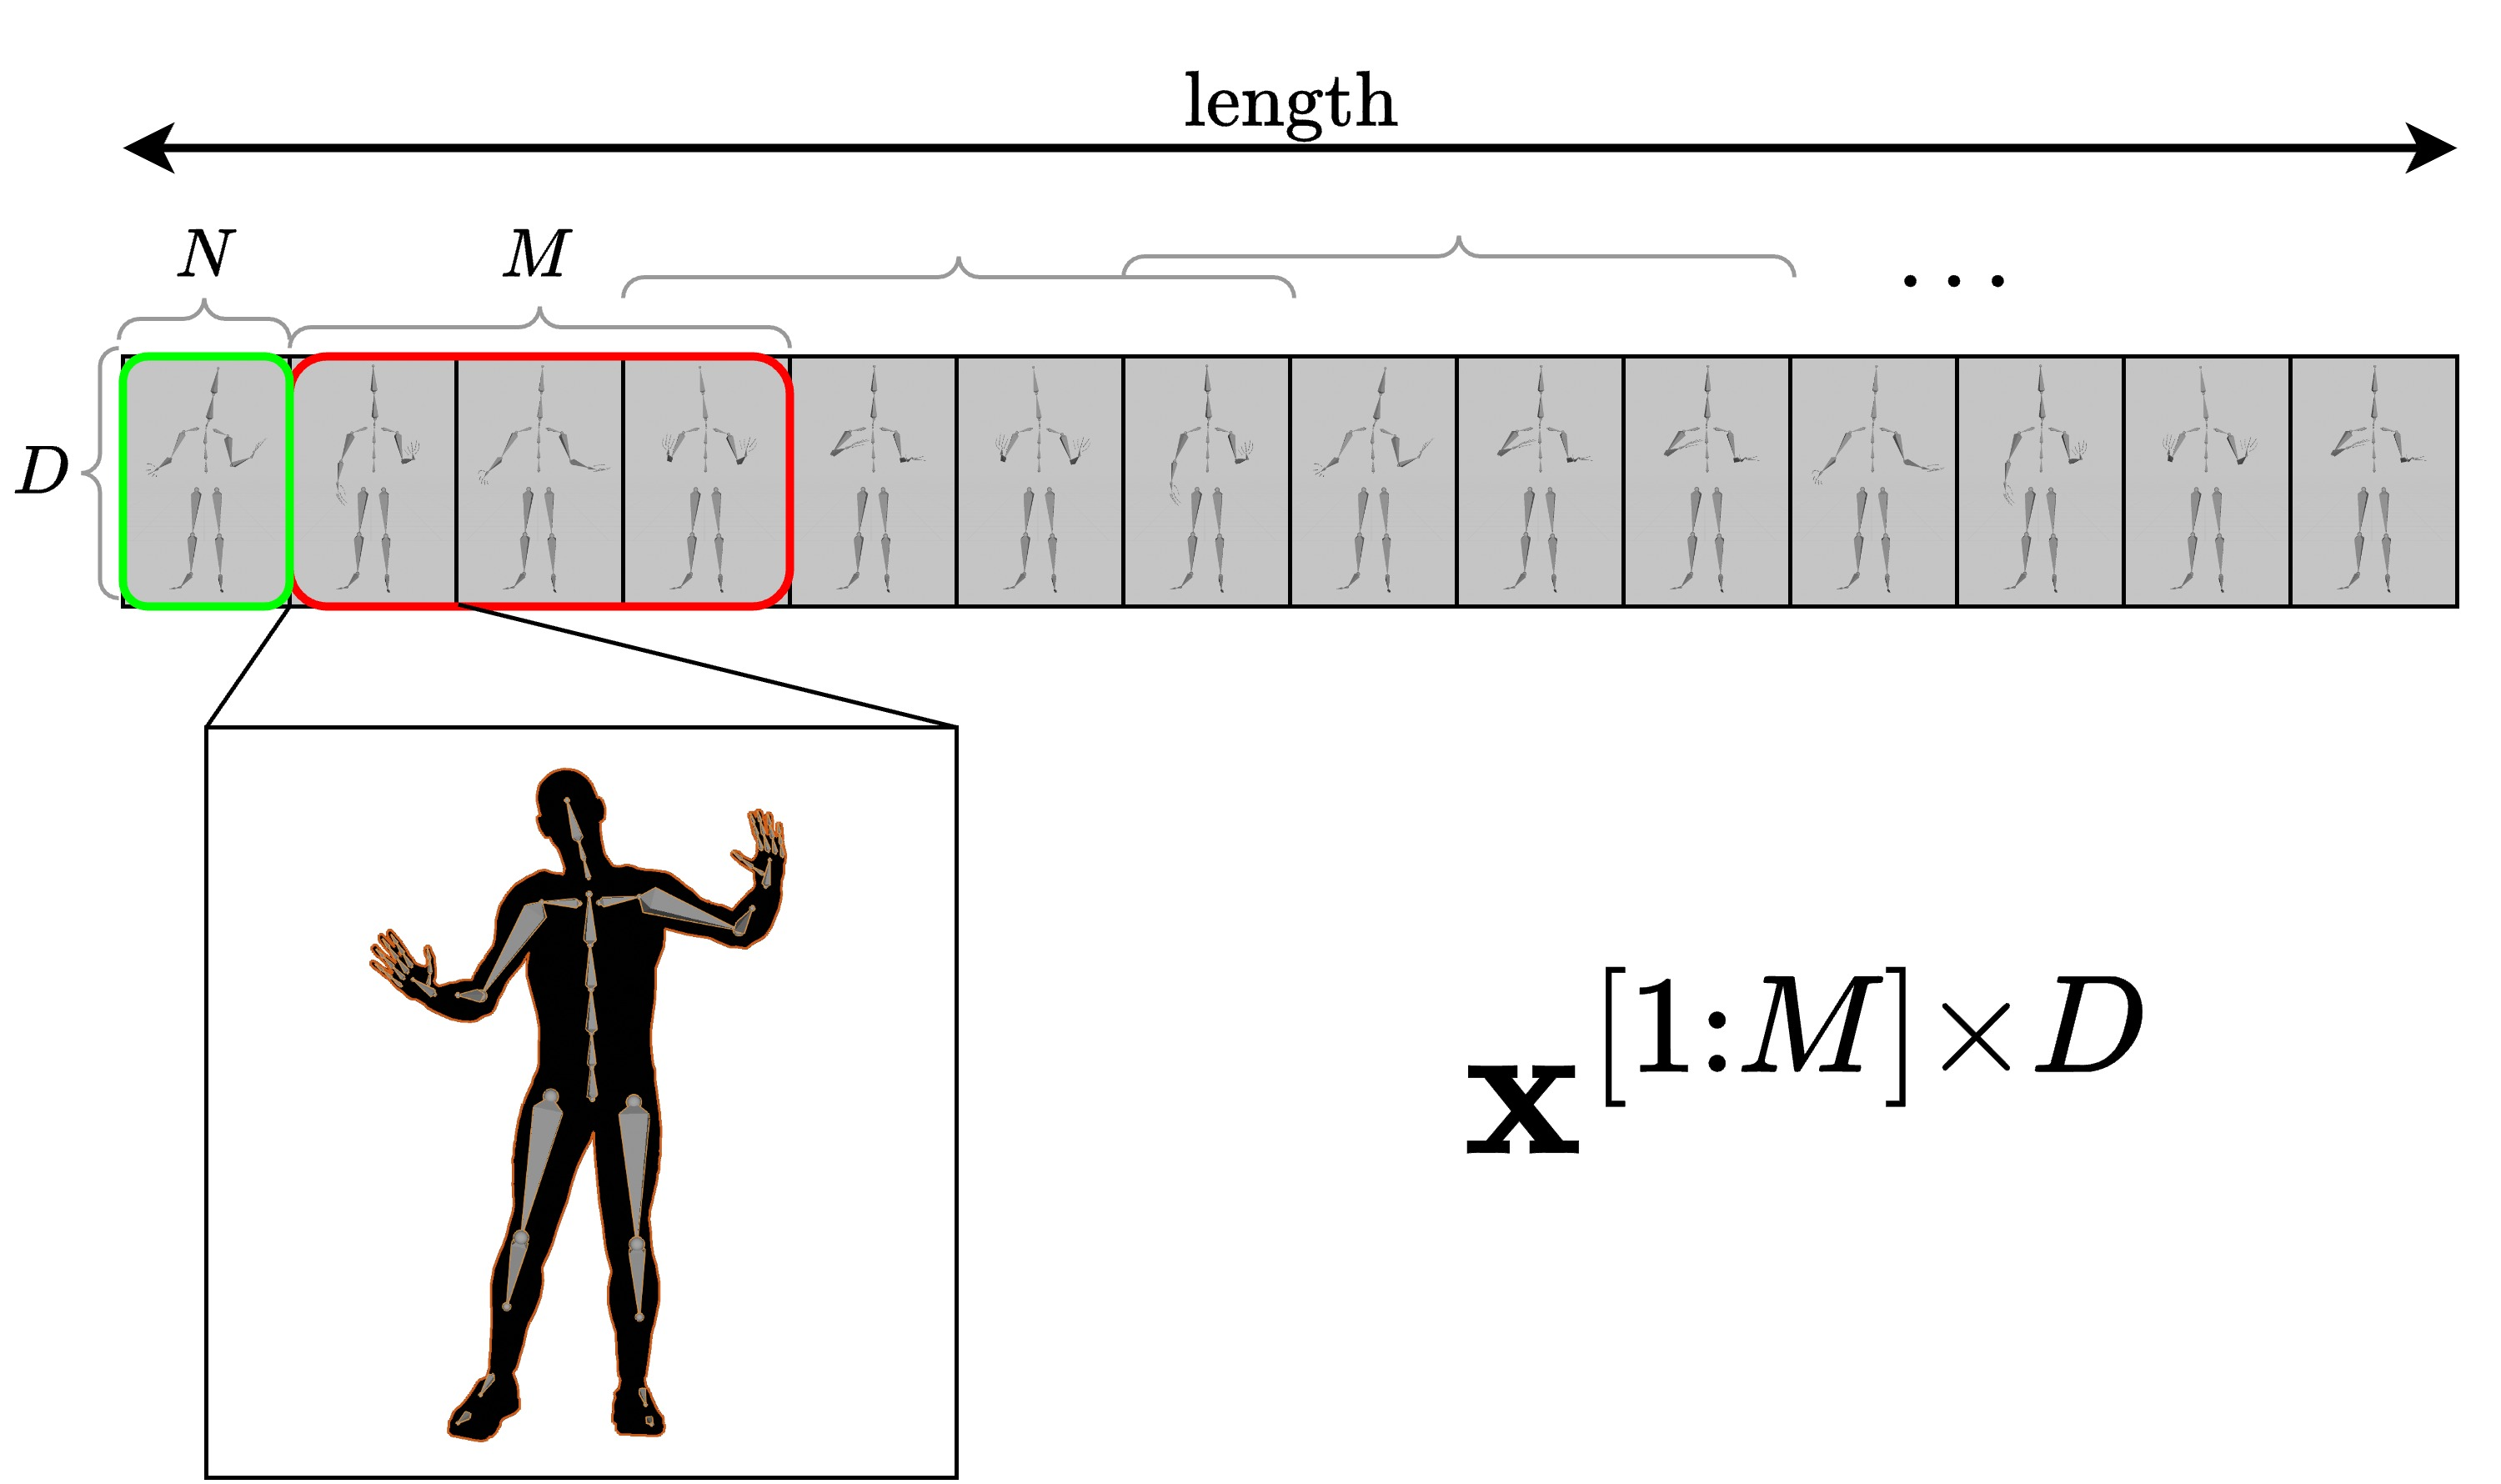
\includegraphics[width=\textwidth]{GestureFrame}
	\end{figure}
	
%{\large 
\begin{equation*}
\mathbf{g}^{[1:\operatorname{length}] \times 75 \times 6} \xrightarrow{ \text{Xử lý} }  \mathbf{g}^{[1: \operatorname{length}] \times D} \xrightarrow{ \text{Cắt} } \mathbf{g}^{[N + M] \times D}
\end{equation*}

%\textbf{Dữ liệu}
%{\Large
%	\begin{equation*}
%		\mathbf{x}^{[1:M] \times D}
%	\end{equation*}
%}

%\begin{itemize}
%	\item $[1:M]$: từ frame $1$ đến frame thứ $M$
%	\item Mỗi frame chứa đặc trưng $D$
%	%				$D = 1141$
%\end{itemize}
\end{frame}



\begin{frame}{Phát biểu bài toán}
%	\begin{figure}[h]
%		\centering
%		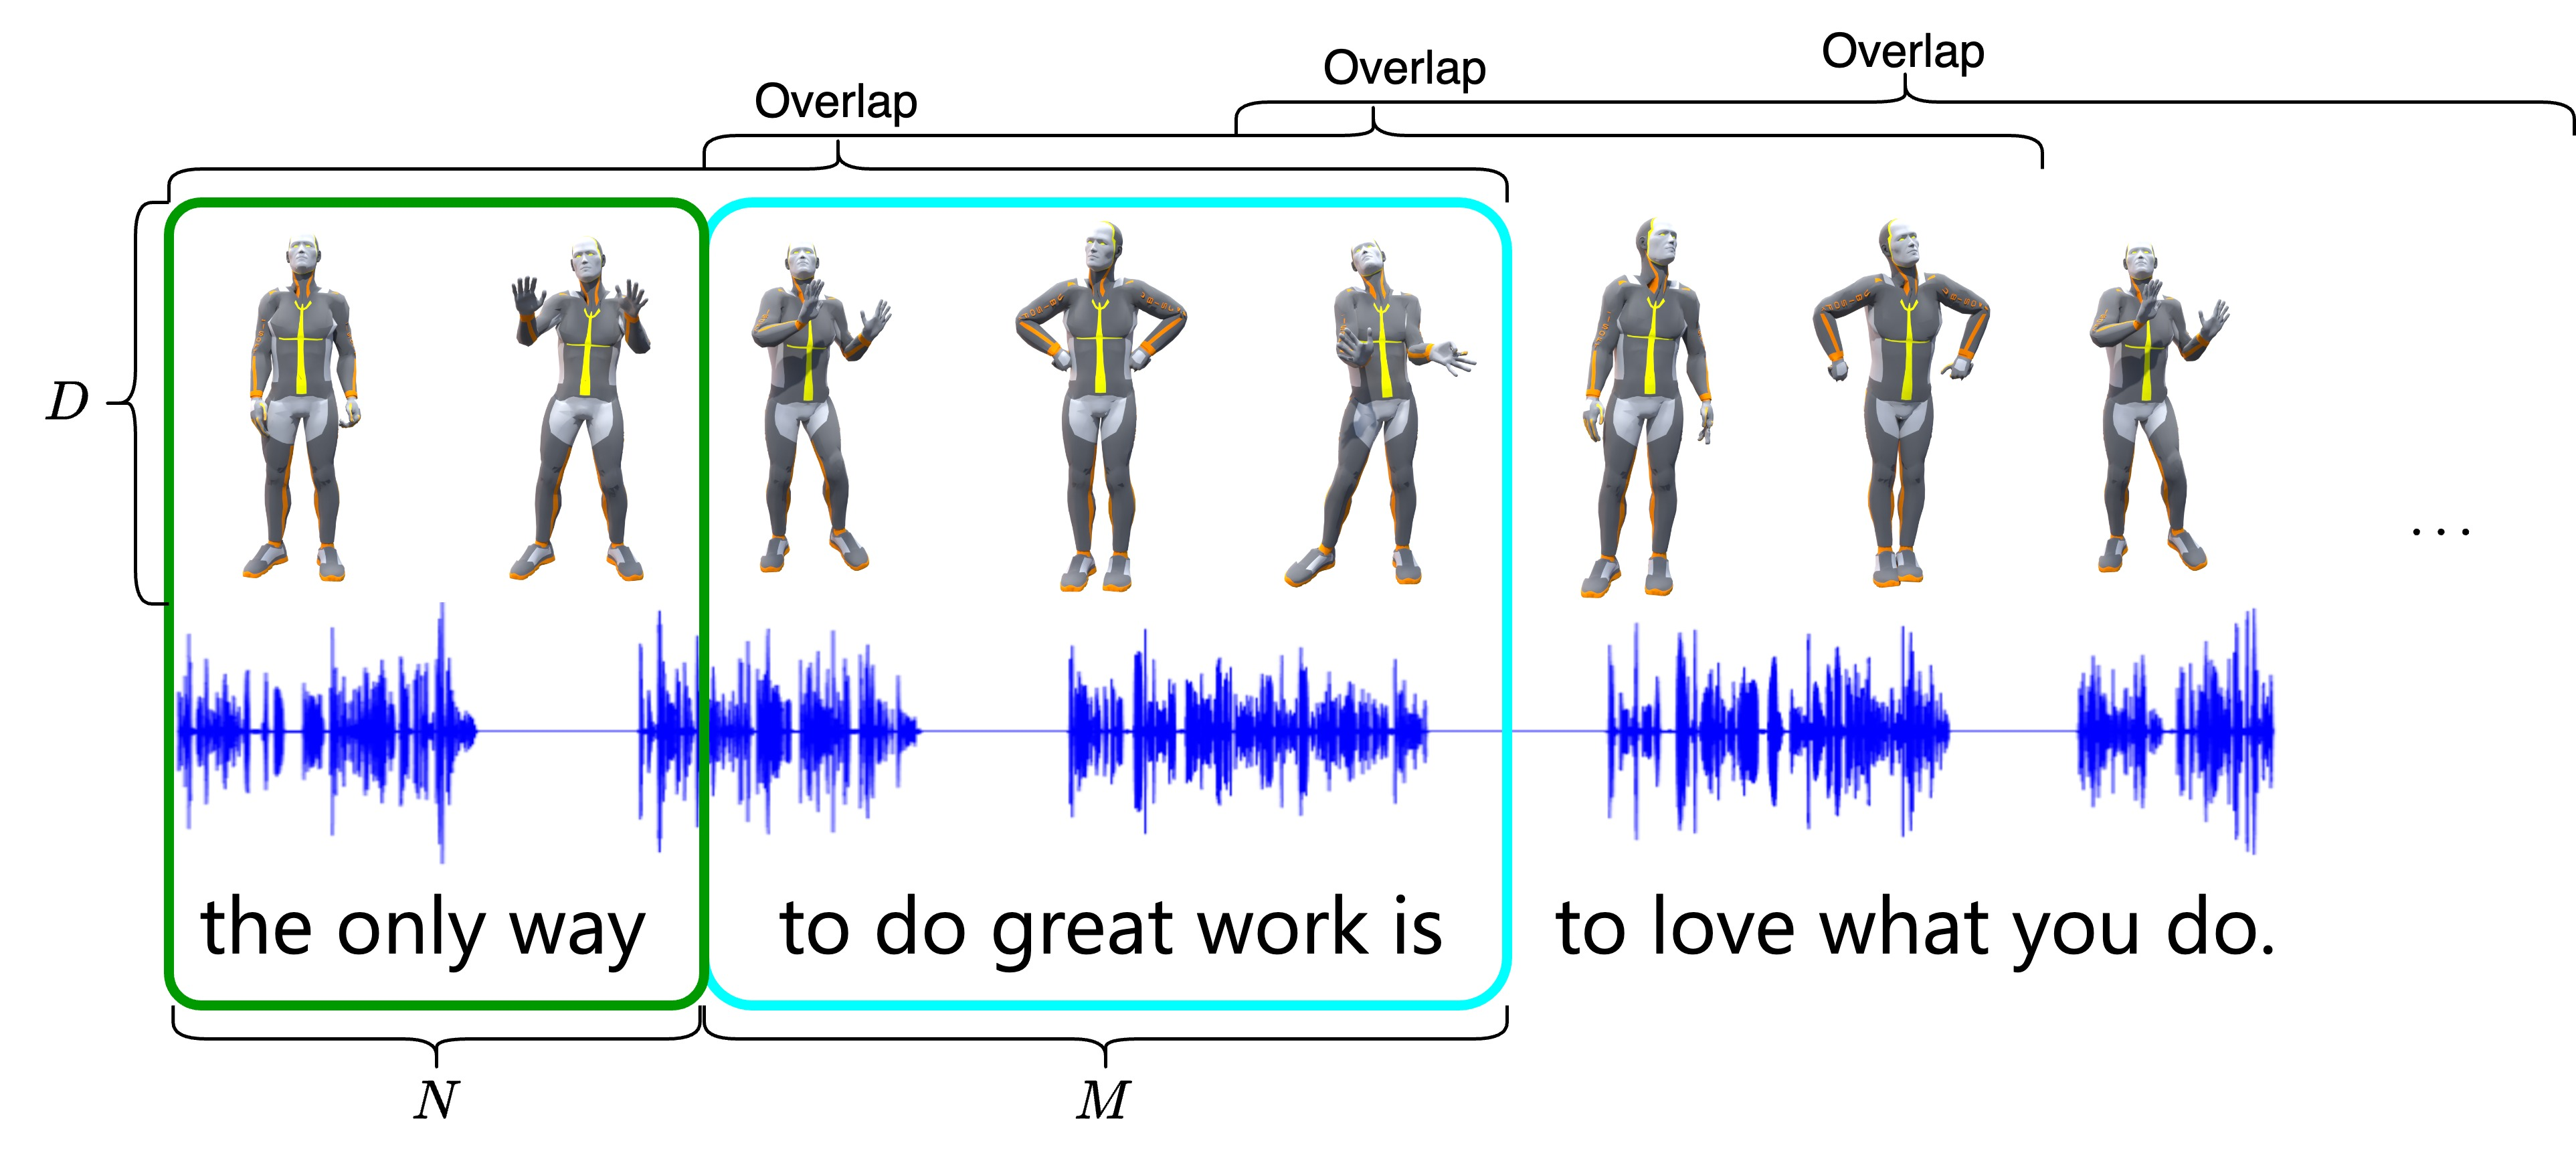
\includegraphics[height=4.5cm]{GestureSeries}
%	\end{figure}
 \vspace{-25pt}
	\begin{figure}
		\centering
		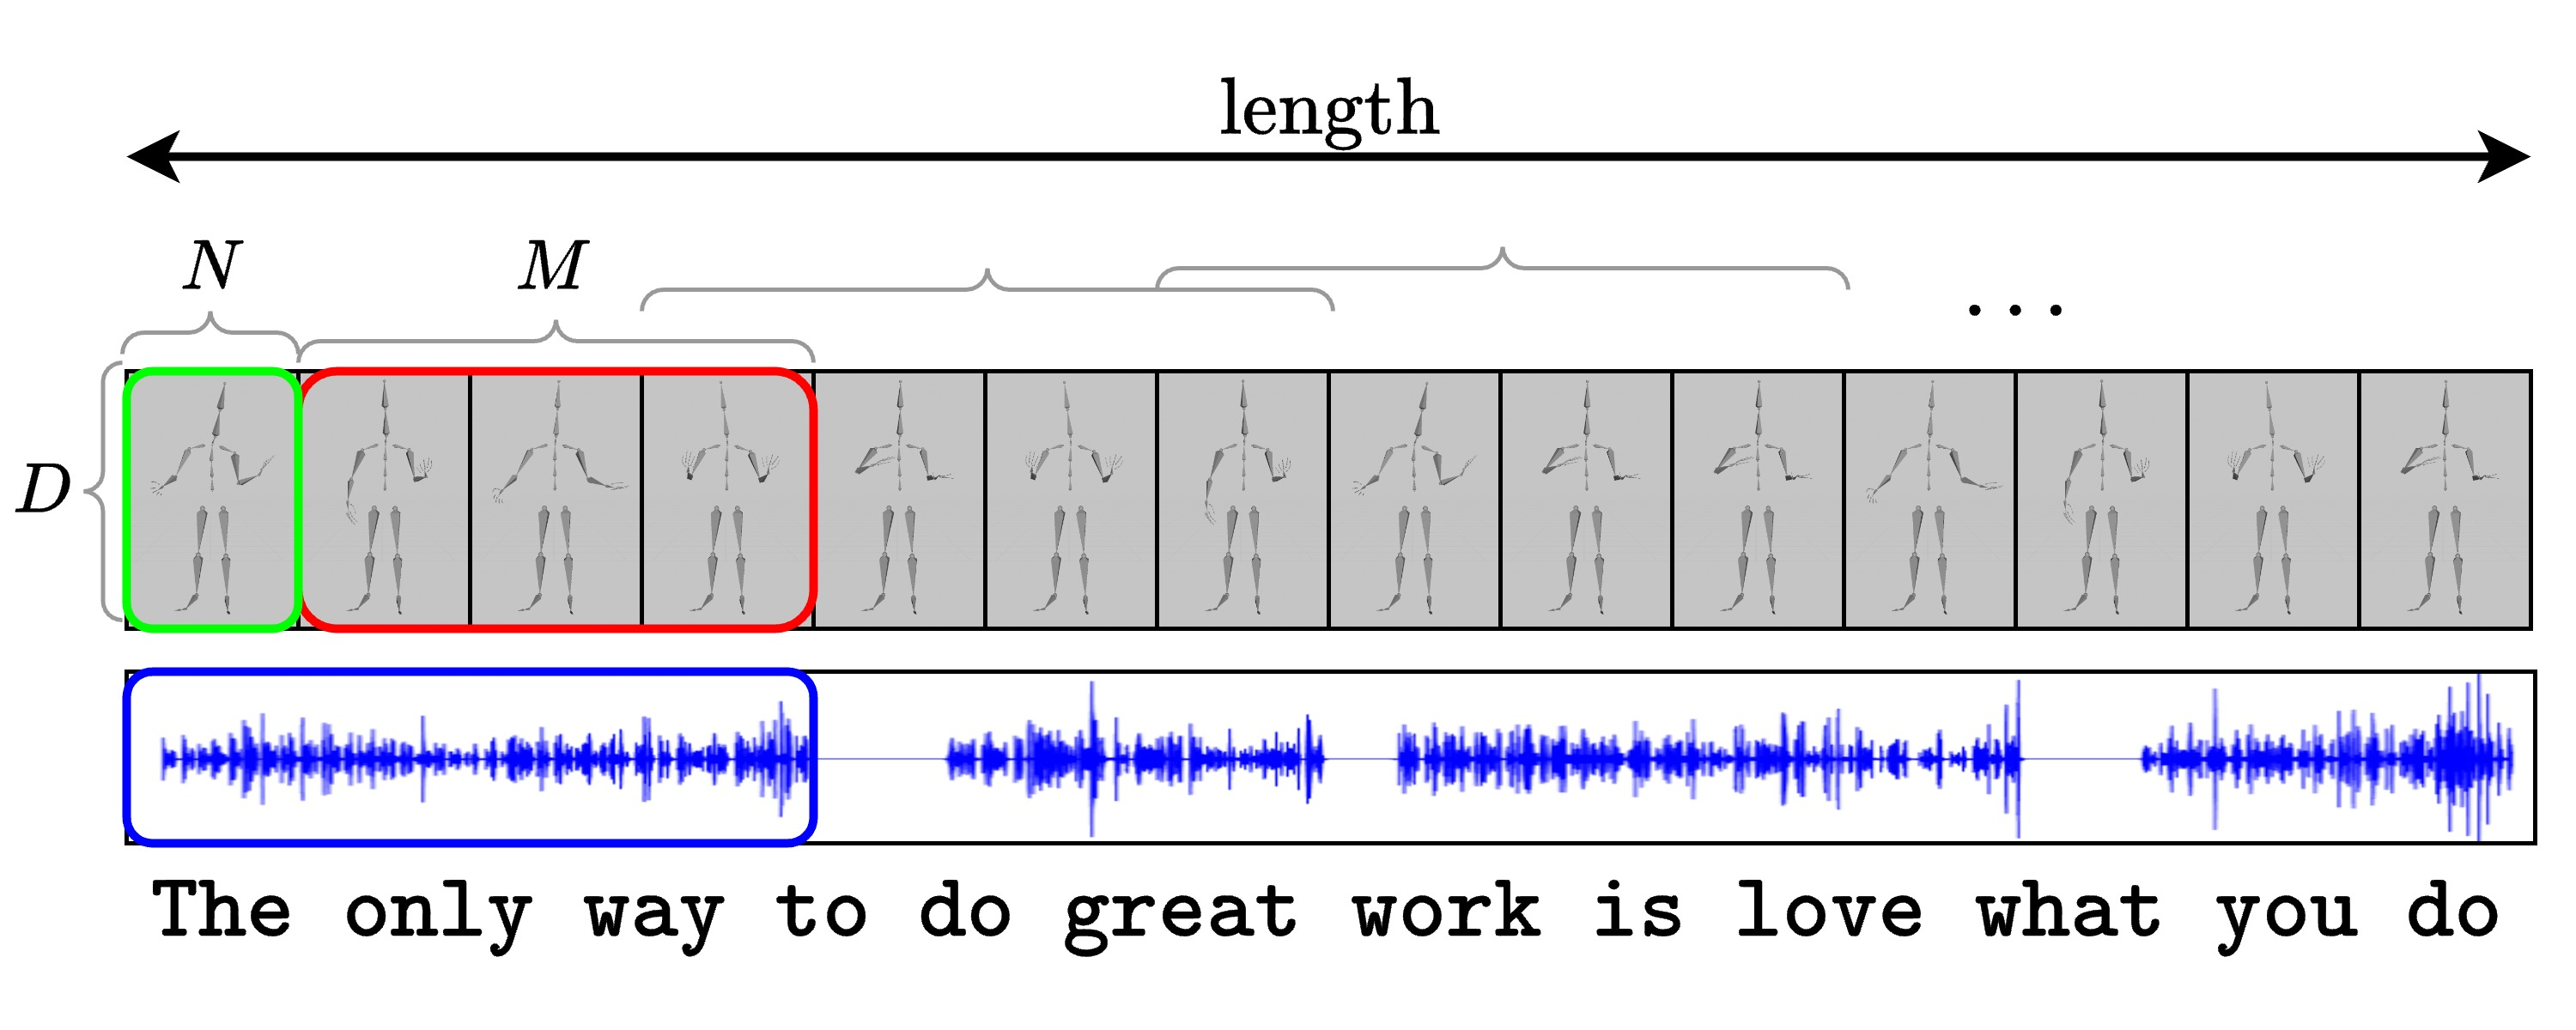
\includegraphics[width=0.95\textwidth]{FeatureProcessing}
	\end{figure}
		\vspace{20pt}
	\begin{columns}
		
	\begin{column}{0.6\textwidth}
		
		\textbf{Input}
		\begin{itemize}
			\item Chuỗi cử chỉ khởi tạo: $\mathbf{s} \in \mathbb{R}^{[1:N] \times D}$
			\item Chuỗi âm thanh: $\mathbf{a}$
			\item Văn bản: $\mathbf{v}$ 
%				\in \mathbb{R}^{16000 M}
			%			trích xuất đặc trưng MFCC: $\mathbf{a} \in \mathbb{R}^{M \times C_{\text{mfcc}}}$
			\item Cảm xúc: $\mathbf{e}$ 
			
			{\small
				(\texttt{Happy},  \texttt{Sad},  \texttt{Neutral}, \texttt{Angry}, \texttt{Old}, \texttt{Funny})
			}
%				 $\text{"Love what you do"}$
		\end{itemize}
		
	\end{column}

	\begin{column}{0.4\textwidth}
		\textbf{Output}
		\begin{itemize}
			\item Chuỗi cử chỉ dự đoán: $\hat{\mathbf{x}} \in \mathbb{R}^{[1:M] \times D}$
		\end{itemize}
		
		\textbf{Grouth Truth}
		\begin{itemize}
			\item Chuỗi cử chỉ gốc: $ \mathbf{x}  \in \mathbb{R}^{[1:M] \times D}$
		\end{itemize}
	\end{column}
\end{columns}
	
\end{frame}




\begin{frame}{Các công đoạn}
	\begin{figure}[h]
		\centering
		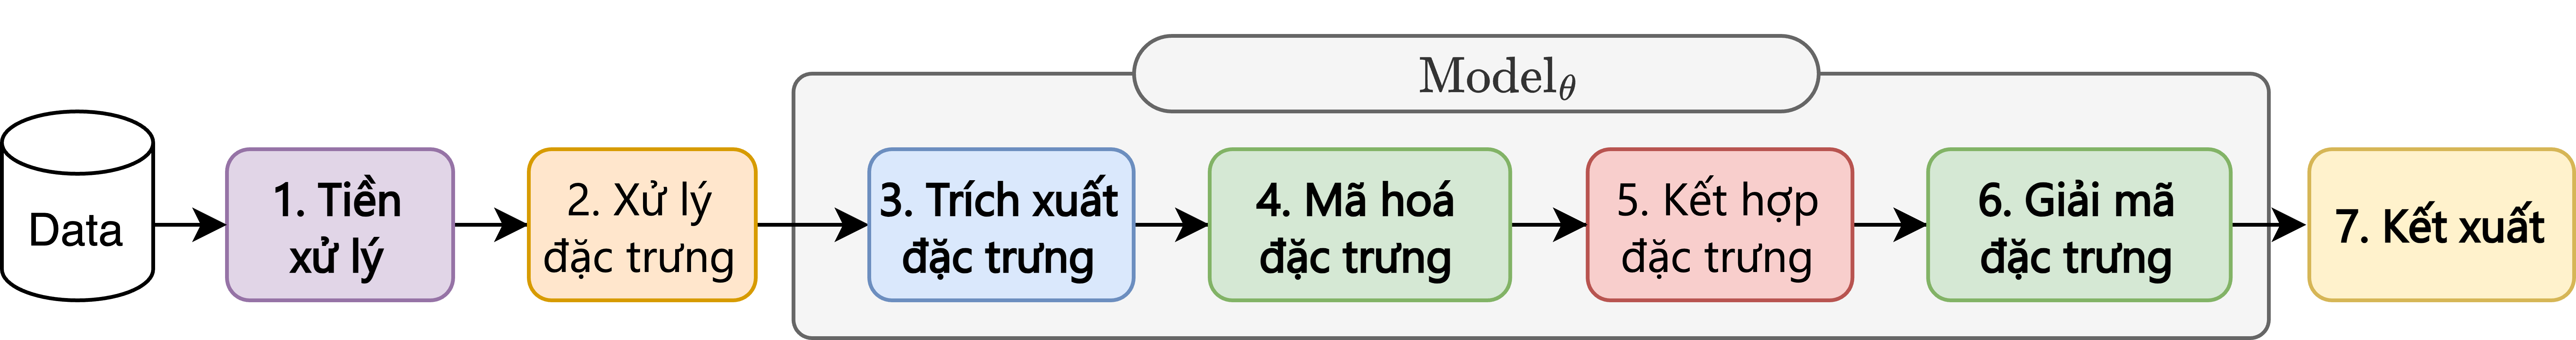
\includegraphics[width=\textwidth]{TotalStage}
	\end{figure}
\end{frame}


\begin{frame}{Công đoạn 1: Tiền xử lý dữ liệu}
%	\begin{equation*}
%		\mathbf{g} \in \mathbb{R}^{[1: \text{length} ] \times (75 \times {\{p_x, p_y, p_z, r_x, r_y, r_z\}})} \xrightarrow{\text{pre-processing}}  \mathbb{R}^{[1: \text{length}] \times D}
%	\end{equation*}
	\begin{figure}
		\centering
		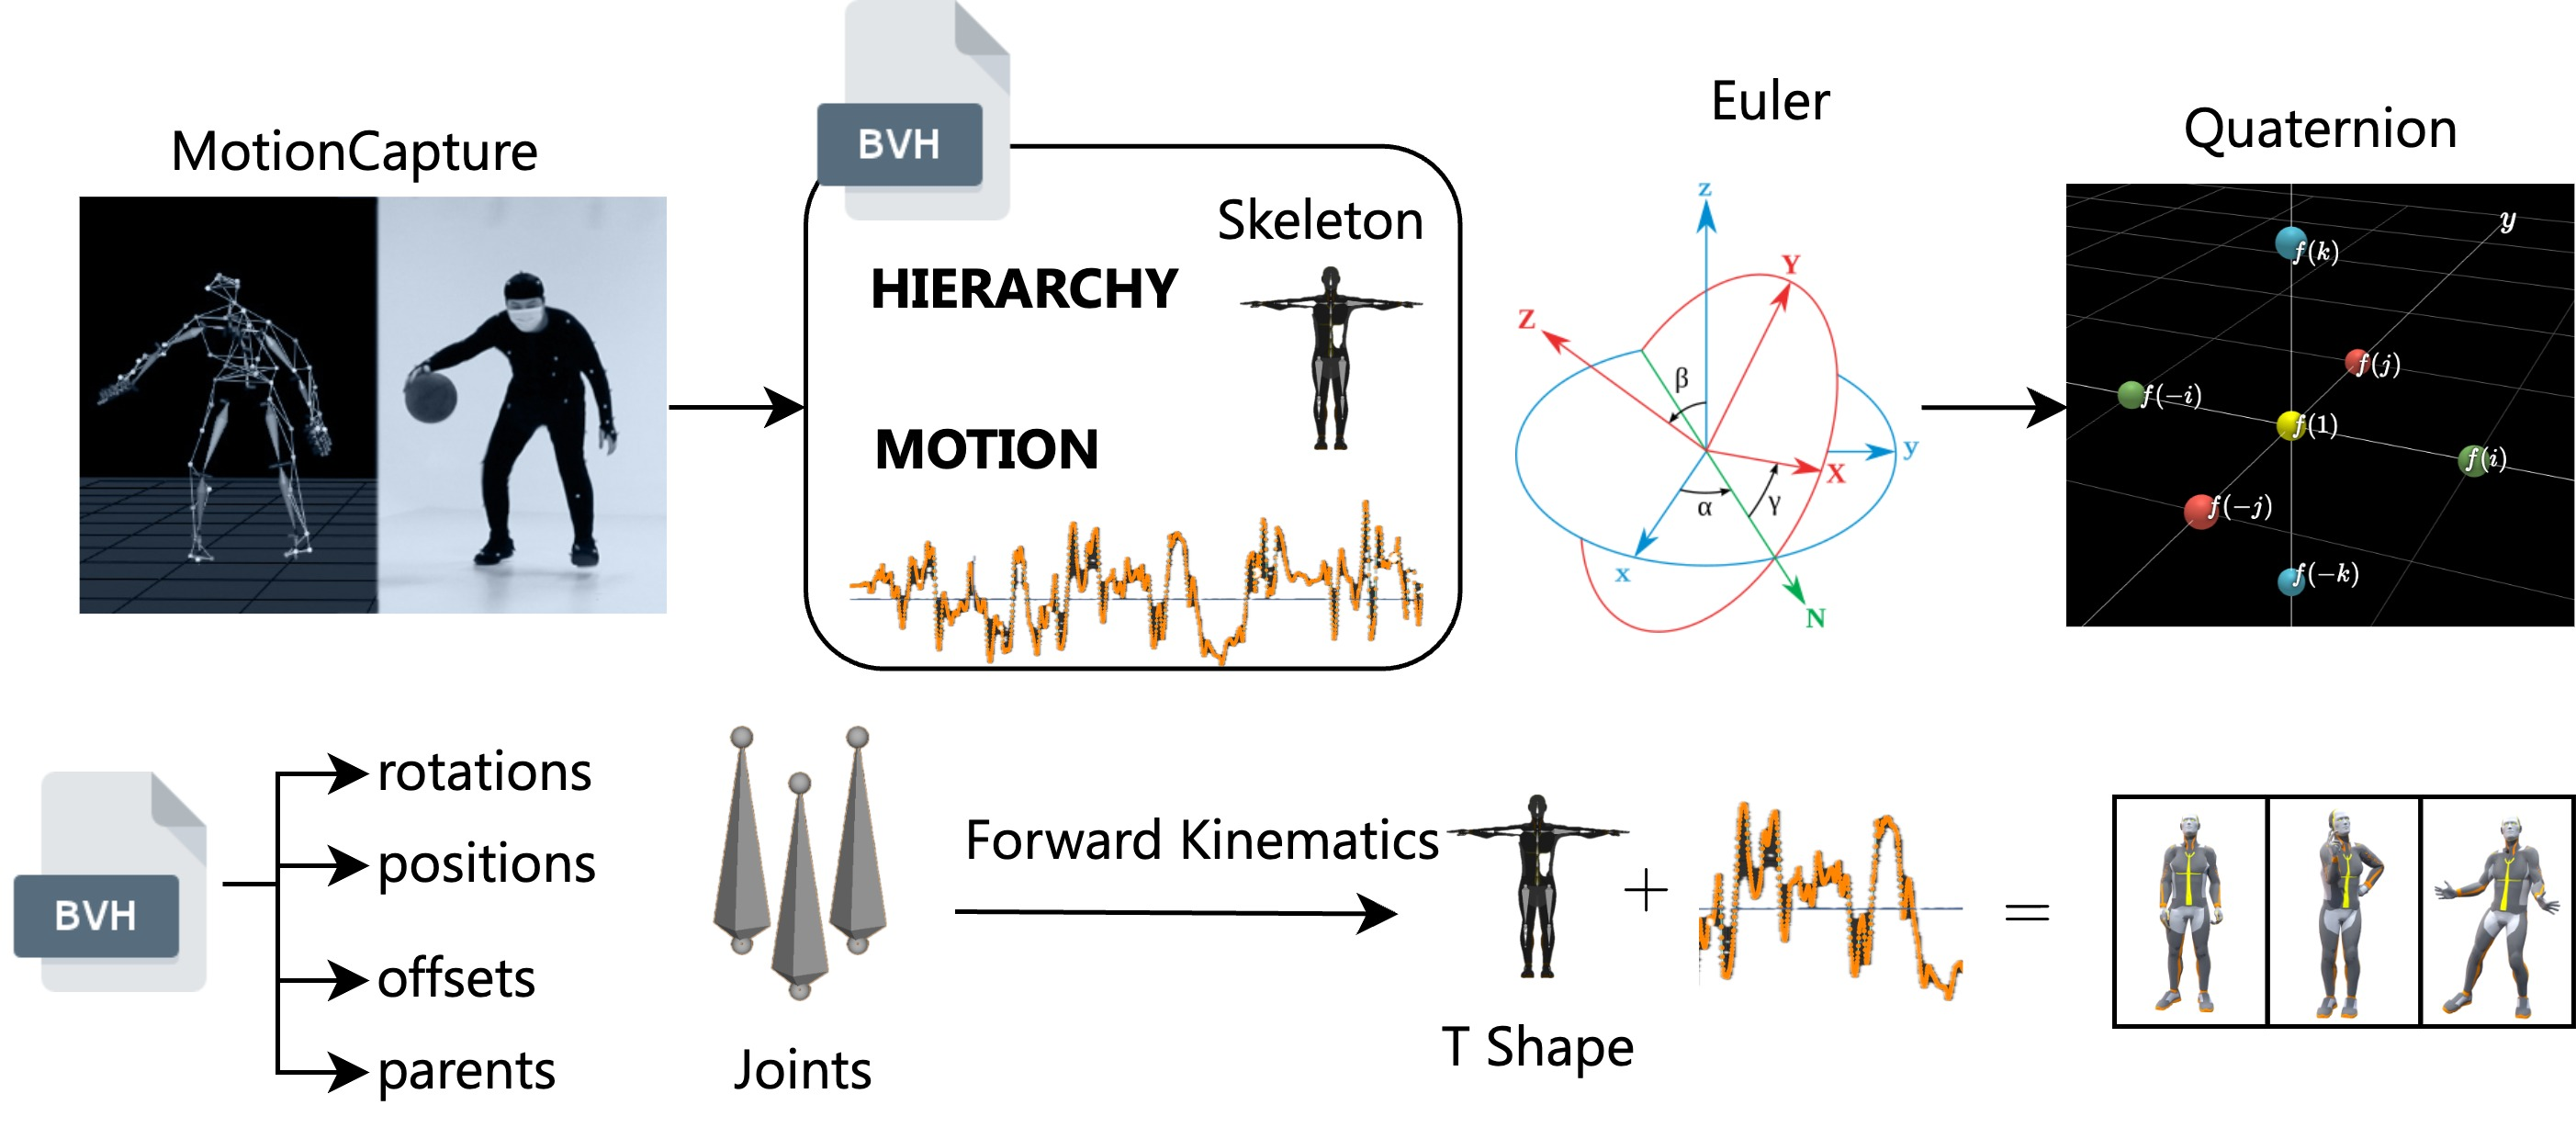
\includegraphics[width=\textwidth]{Preprocessing}
	\end{figure}
	
\end{frame}



\begin{frame}{Đặc trưng dữ liệu của $1$ frame}
	\begin{figure}
		\centering
		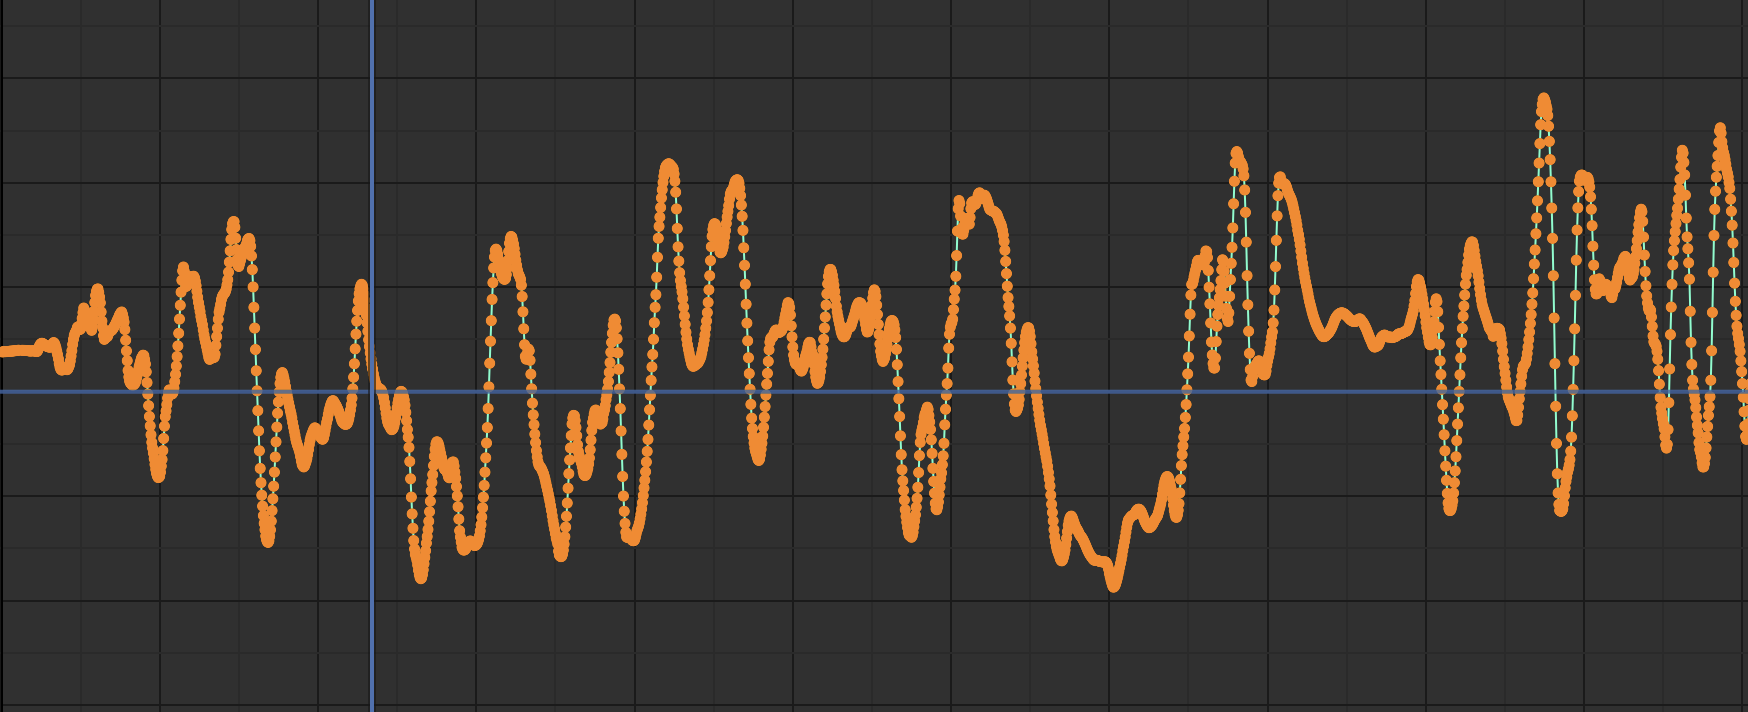
\includegraphics[width=\textwidth, height=60pt]{MotionXYZ.png}
		%		\caption{Minh hoạ chuyển động của góc quay một xương trong toạ độ}
	\end{figure}
	\begin{equation}
		\mathbf{g}^{[1]} = \Big[ \mathbf{p}_{\text{root}},  \mathbf{r}_{\text{root}},
		\mathbf{ p }'_{\text{root}},  \mathbf{r}'_{\text{root}},
		\mathbf{p}_{\text{joins}},  \mathbf{r}_{\text{joins}},
		\mathbf{p}'_{\text{joins}},  \mathbf{r}'_{\text{joins}},
		\mathbf{d}_{\text{gaze}}
		\Big]
	\end{equation}
	\vspace{-10pt}
	
	{\small
		\begin{itemize}
			\item $\mathbf{p}_{\text{root}} \in \mathbb{R}^3$, $\mathbf{r}_{\text{root}} \in \mathbb{R}^4$: Toạ độ và góc quay của điểm gốc
			\item $\mathbf{p}'_{\text{root}} \in \mathbb{R}^3$, $\mathbf{r}'_{\text{root}} \in \mathbb{R}^3$: Vận tốc thay đổi của toạ độ và góc quay gốc
			%		\item : quay
			%		Vận tốc thay đổi của góc quay gốc
			\item $\mathbf{p}_{\text{joins}} \in \mathbb{R}^{3 n_{\text{join} }}$, $\mathbf{r}_{\text{joins}} \in \mathbb{R}^{6 n_{\text{join} }}$: Toạ độ và góc quay của các khung xương
			%		\item : Góc quay của các khung xương
			\item $\mathbf{p}'_{\text{joins}} \in \mathbb{R}^{3n_{\text{join} }}$ và $\mathbf{r}'_{\text{joins}} \in \mathbb{R}^{3n_{\text{join} }}$: Vận tốc thay đổi của toạ độ và góc quay khung xương
			%		\item $\mathbf{r}'_{\text{joins}} \in \mathbb{R}^{3n_{\text{join} }}$: Vận tốc thay đổi của góc quay khung xương
			\item $\mathbf{d}_{\text{gaze}} \in \mathbb{R}^3$: Là hướng nhìn
	\end{itemize}}
	\vspace{-10pt}
	{\small
		\begin{equation*}
			D = 3 + 4 + 3 + 3 + 3 \times 75 + 6 \times 75 + 3 \times 75 + 3 \times 75 + 3 = 1141
	\end{equation*}}
	%	\begin{columns}
		%		\begin{column}{0.78\textwidth}
			
			%			$$
			%			D = 1141
			%			$$
			
			%		\end{column}
		%		
		%		\begin{column}{0.22\textwidth}
			%			\vspace{12pt}
			%			\begin{figure}
				%				\centering
				%				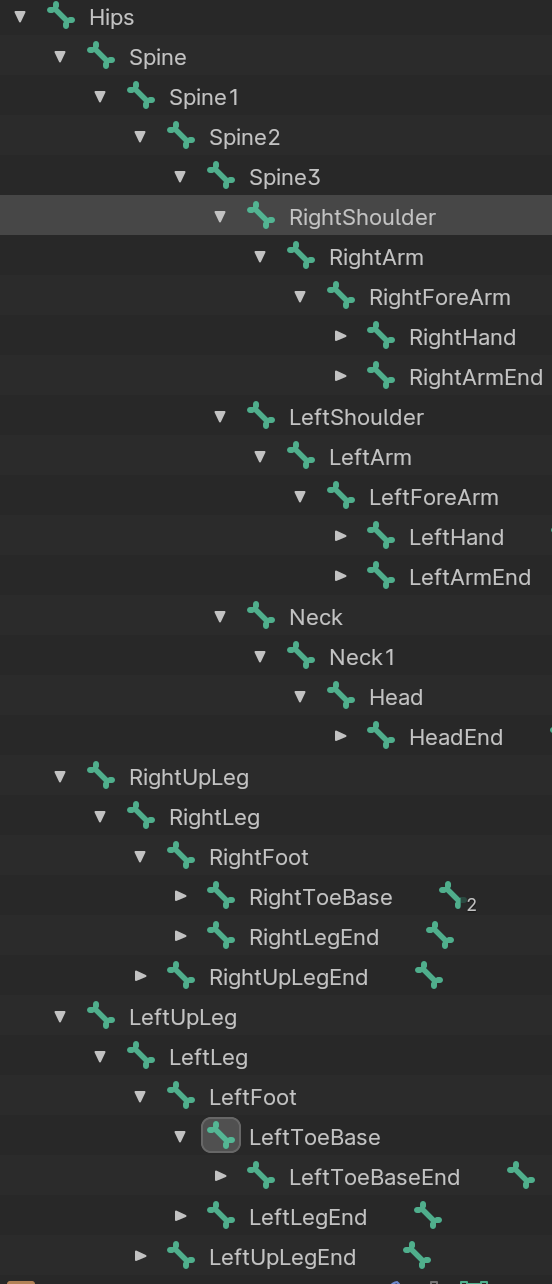
\includegraphics[width=\textwidth]{Bone.png}
				%			\end{figure}
			%			
			%		\end{column}
		%	\end{columns}
	
\end{frame}




\begin{frame}{Thách thức của bài toán}
	
	%	\begin{columns}
		%		\begin{column}{0.55\textwidth}
			%			
			%			
			%			%		\textit{Mô hình Diffusion}:
			%			%		\begin{itemize}
				%				%			\item Ít yêu cầu về dữ liệu gắn nhãn
				%				%			\item Khả năng tương tác và điều chỉnh dễ dàng
				%				%			\item Tính ổn định cao
				%				%		\end{itemize}
			%		\end{column}
		%		\begin{column}{0.45\textwidth}
			%			
			%			\begin{columns}
				%				\begin{column}{0.5\textwidth}
					%					\begin{figure}
						%						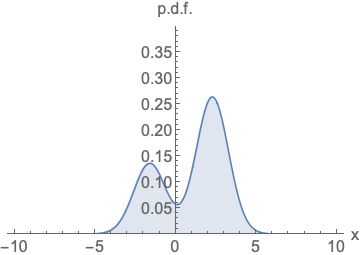
\includegraphics[width=\textwidth]{ProbabilityDensityFunctions.png}
						%						\caption{\scriptsize Phải chuẩn hoá (diện tích dưới đường cong phải tích phân thành một)}
						%					\end{figure}
					%				\end{column}
				%				\begin{column}{0.5\textwidth}
					%					\begin{figure}
						%						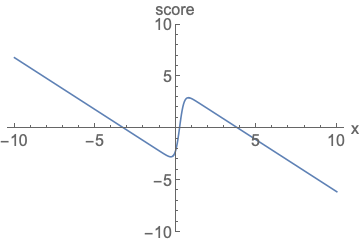
\includegraphics[width=\textwidth]{ScoreFunction.png}
						%						\caption{\scriptsize Không cần chuẩn hoá.}
						%					\end{figure}
					%				\end{column}
				%			\end{columns}
			%			
			%			
			%			
			%			\begin{columns}
				%				\begin{column}{0.5\textwidth}
					%					\centering
					%					\begin{tikzpicture}
						%						\node at (0, 1) {$p(\mathbf{x})$};
						%						
						%						\node at (0, 0.5) {\small \text{probability density}};
						%						
						%						\draw[<->, thick] (0, 0) -- (0, -0.5);
						%						
						%						\node at (0, -1) {$\nabla_\mathbf{x} \log p(\mathbf{x})$};
						%						
						%						\node at (0, -1.5) {\small \text{score function}};
						%					\end{tikzpicture}
					%					
					%				\end{column}
				%				\begin{column}{0.5\textwidth}
					%					\begin{figure}
						%						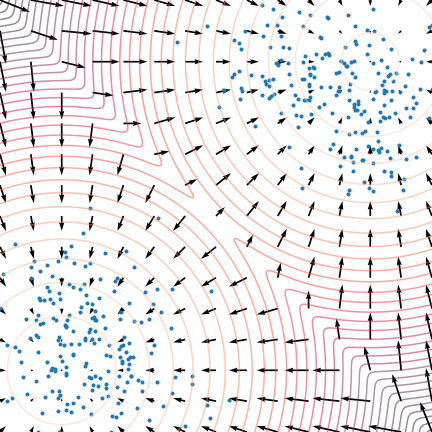
\includegraphics[width=\textwidth]{CompareScoreFunction.png}
						%						\caption{\scriptsize score function vs probability density}
						%					\end{figure}
					%				\end{column}
				%			\end{columns}
			%		\end{column}
		%	\end{columns}
	\textbf{Quan hệ giữa dữ liệu cử chỉ và âm thanh}:
	\begin{itemize}
		\item Quan hệ n:n của âm thanh, cử chỉ, cảm xúc.
	\end{itemize}
	%		Baseline: \textbf{MDM}  (Human Motion Diffusion Model)
	\textbf{Khó khăn}
	\begin{enumerate}
		\item Dữ liệu không đủ nhiều và chất lượng, chi phí cao
		\item Không cân xứng về dữ liệu giữa các loại đăng trưng cần học (âm thanh, cử chỉ)
		\item Thiếu đồng nhất của về ngữ cảnh của các loại dữ liệu
		%				\item Quá trình sinh có thể dể điều khiển 
		%			hơn GAN.
	\end{enumerate}
	%	$\rightarrow$  \textbf{DiffuseStyleGesture}: Diffusion cho bài toán sinh cử chỉ
\end{frame}


%
%\begin{frame}{Đóng góp}
%
%\end{frame}
%\[
%\begin{array}{ll}
%\mbox{minimize} & f(x) + \lambda \sum_{i=1}^N \|x_i\|_2
%\end{array}
%\]


%\begin{frame}{Structured group lasso \\[-0.3em] 
%{\footnotesize \textmd{(Jacob, Obozinski, Vert; Bach et al.; Zhao, Rocha, Yu; \dots)}}}
%\begin{itemize}\itemsep=12pt
%\item problem:
%\[
%\begin{array}{ll}
%\mbox{minimize} & f(x) + \sum_{i=1}^N \lambda_i \|x_{g_i}\|_2
%\end{array}
%\]
%where $g_i \subseteq [n]$ and $\mathcal G = \{g_1, \dots, g_N\}$
%\item like group lasso, but the groups can overlap arbitrarily
%\item particular choices of groups can impose `structured' sparsity
%\item \eg, topic models, selecting interaction terms for (graphical) models,
%    tree structure of gene networks, fMRI data
%\item generalizes to the \textbf{composite absolute penalties family}:
%\[
%r(x) = \|(\|x_{g_1}\|_{p_1}, \dots, \|x_{g_N}\|_{p_N})\|_{p_0}
%\]
%\end{itemize}
%\end{frame}

%\begin{frame}{Structured group lasso \\[-0.3em] 
%{\footnotesize \textmd{(Jacob, Obozinski, Vert; Bach et al.; Zhao, Rocha, Yu; \dots)}}}
%\textbf{hierarchical selection}:
%\begin{center}
%\begin{tikzpicture}
%[dot/.style={rectangle,draw=black,fill=white,inner sep=5pt,minimum size=5pt}]
%\node[dot,draw=orange,thick] at (0,5) (n1) {1};
%\node[dot] at (-1,4) (n2) {2};
%\node[dot,draw=orange,thick] at (1,4) (n3) {3};
%\node[dot] at (-1,3) (n4) {4};
%\node[dot,draw=orange,thick] at (0.5,3) (n5) {5};
%\node[dot] at (1.5,3) (n6) {6};
%\draw[->] (n1) -- (n2);
%\draw[->] (n1) -- (n3);
%\draw[->] (n2) -- (n4);
%\draw[->] (n3) -- (n5);
%\draw[->] (n3) -- (n6);
%\end{tikzpicture}
%\end{center}
%\begin{itemize}\itemsep=8pt
%    \item $\mathcal G = \{ \{4\}, \textcolor{orange}{\{5\}}, \{6\}, \{2,4\}, 
%        \textcolor{orange}{\{3,5,6\}}, \textcolor{orange}{\{1,2,3,4,5,6\} \}}$
%\item nonzero variables form a rooted and connected subtree
%    \begin{itemize}
%        \item if node is selected, so are its ancestors
%        \item if node is not selected, neither are its descendants
%    \end{itemize}
%\end{itemize}
%\end{frame}

%\begin{frame}[fragile]{Sample ADMM implementation: lasso}
%\begin{verbatim}
%prox_f = @(v,rho) (rho/(1 + rho))*(v - b) + b;
%prox_g = @(v,rho) (max(0, v - 1/rho) - max(0, -v - 1/rho));
%
%AA = A*A';
%L  = chol(eye(m) + AA);
%
%for iter = 1:MAX_ITER
%    xx = prox_g(xz - xt, rho);
%    yx = prox_f(yz - yt, rho);
%
%    yz = L \ (L' \ (A*(xx + xt) + AA*(yx + yt)));
%    xz = xx + xt + A'*(yx + yt - yz);
%  
%    xt = xt + xx - xz;
%    yt = yt + yx - yz;
%end
%\end{verbatim}
%\end{frame}